% Missing putting everything together
% Add at the very end comparing ref_qr to new_qr
\documentclass[12pt]{beamer}
\title{Optimized Computation of the Q Factor in LAPACK}
\author{Johnathan Rhyne\\Advised by: Julien Langou}
\institute{University of Colorado Denver}
\usepackage{algorithm}
\usepackage{algpseudocode}
\usepackage{multicol}
\usepackage{environ}
\usepackage{tikz}
\usetikzlibrary{shapes.geometric}
\date{\today}

\newcommand{\customframefont}[1]{
\setbeamertemplate{itemize/enumerate body begin}{#1}
\setbeamertemplate{itemize/enumerate subbody begin}{#1}
}

\NewEnviron{framefont}[1]{
\customframefont{#1} % for itemize/enumerate
{#1 % For the text outside itemize/enumerate
\BODY
}
\customframefont{\normalsize}
}

\newcommand{\R}{\mathbb{R}}


%---------------%
% Abstract:     %
%---------------%
% Computing the Q Factor is an important operation for some applications and end users, so 
%  we aim to demonstrate new algorithms can speed up the performance of these operations for
%  end users. We implement existing algorithms 
%  originally developed by [insert authors here]. We see performance improvements on
%  the order of [insert rought value here] in comparison to the reference LAPACK 
%  computations and see similar performance in many cases as the optimized implementation
%  for AMD (AOCL). Using these schemes we not only see an improvement in execution time,
%  but lowers the memory footprint for the main driver algorithm.
%
%
%

\begin{document}
    \begin{frame}
        \titlepage
    \end{frame}
    % Table of contents. Can be helpful for navigating after the fact
    \begin{framefont}{\small}
    \begin{frame}
        \frametitle{Overview}
        \begin{multicols}{2}
            \tableofcontents
        \end{multicols}
    \end{frame}
    \end{framefont}
    \section{Preliminaries}
    \begin{frame}
        %
        %LAPACK stands for Linear Algebra PACKage, which provides a suite of routines to 
        %perform many linear algebra operations including but not limited to:
        %
        \frametitle{What is LAPACK}
        LAPACK provides interfaces for:
        \begin{enumerate}
            \item Matrix multiplication
            \item Solving linear systems of equations
            \item Factorizing matrices
        \end{enumerate}
        and more!
        %
        %We provide the interface and then set a baseline for chip vendors like INTEL and AMD to either package
        %or beat themselves.
        %
    \end{frame}
    \begin{frame}
        \frametitle{Notation}
        Throughout this presentation we will use the notation used by LAPACK. The first character determines what kind of numbers we are working with. Ex:
        \begin{itemize}
            \item DLACPY is the routine that copies double precision real numbers from one matrix to another
        \end{itemize}
        In this presentation, we will be restricting our discussion to only double precision real numbers,
        but there are analogous versions for single precision real, and both complex precisions.
    \end{frame}
    \begin{frame}
        \frametitle{Brief Linear Algebra Review}
        Householder reflectors are a way to to represent a matrix as a product of rank $1$ updates of the form
        $$
            Q = \left(I - \tau_1 v_1v_1^\top\right)\cdots\left(I - \tau_k v_kv_k^\top\right) = I - VTV^\top
        $$
        Routines that use this\footnote{Collected by listing some functions found on the caller graph of DLARFT found \textcolor{blue}{\href{https://netlib.org/lapack/explore-html//d7/d0d/group__larft_ga20e5a4f351b3ca7d30078547e55884f5_ga20e5a4f351b3ca7d30078547e55884f5_icgraph_org.svg}{here}}}
        \begin{itemize}
            \item SVD *GESVD
            \item Hessenberg Reduction *GEBRD
            \item QR Factorization *GEQRF
        \end{itemize}
    \end{frame}
    \section{DORGQR Overview}
    \subsection{Motivation}
    \begin{frame}
        \frametitle{Basic Algorithm}
            In order to compute this matrix, we can do the following.\\\,\\
        \begin{algorithmic}[1]
            \State Initialize $Q$ to $I$.
            \For{Each column of $V$ denoted $v_i$ from $i=n$ to $1$}
            \State Apply $I-\tau_iv_iv_i^\top$ to $Q$ from the left
            \EndFor
        \end{algorithmic}\,\\
        This method will give us the answer by applying all of our reflectors one after the other. But, we can make this 
        faster by doing many at the same time!
    \end{frame}
    \subsection{Existing Behavior}
    \begin{frame}
        \frametitle{Blocking algorithm}
        In practice, we don't do one reflector at a time, we do many! The algorithm to do so is as follows\\\,\\
        \begin{algorithmic}[1]
            \State Determine blocking parameter $nb$
            \State Initialize $Q$ as the $m\times m$ identity matrix
            \For{Each block of size $nb$ of $V$}
            \State Compute the $T$ factor
            \State Apply the block of reflectors to trailing columns of $Q$
            \State Apply the block of reflectors to the current block of columns of $Q$
            \EndFor
        \end{algorithmic}
    \end{frame}
    \subsection{Places for Optimization}
    \begin{frame}
        \frametitle{Places for Optimization}
        We have $4$ main places to look at to optimize this computation.
        \begin{enumerate}
            \item Computing $T$ (DLARFT)
            \item Applying to the trailing columns of $Q$ (DLARFB)
            \item Applying to the current window of $Q's$ columns (DORG2R)
            \item Take advantage of initializing $Q$ as $I_m$. (Main driver DORGQR)
        \end{enumerate}
    \end{frame}
    \section{Computation of T}
    \begin{frame}
        \frametitle{Main DLARFT idea}
        % In order to motivate the recursive formulation, we notice that if we had a way to collect these
        % T values for the first l columns and the remaining, we want to do the following
        If we collect only some of the reflectors on the first and second half, we get
        \begin{align*}
            &\,(I - V_1T_{1,1}V_1^\top)(I - V_2T_{2,2}V_2^\top) \\
            &= I - V_1T_{1,1}V_1^\top - V_2T_{2,2}V_2^\top + V_1T_{1,1}V_1^\top V_2T_{2,2}V_2^\top
        \end{align*}
        Can be rewritten as:
        $$
            I - VTV^\top
        $$
        where:
        % Rewrite the T with indices
        % Write T out 
        % Then, if we define T_3 and V as follows, we can recover above!
        \begin{align*}
            T_{1,2} &= -T_{1,1}V_1^\top V_2T_{2,2} \\
            V &= \begin{bmatrix}
                V_1 & V_2
            \end{bmatrix}\\
            T &= \begin{bmatrix}
                T_{1,1} & T_{1,2} \\
                0       & T_{2,2}
            \end{bmatrix}
        \end{align*}
    \end{frame}
    \subsection{Existing Behavior}
    \begin{frame}
        \frametitle{LAPACK Implementation}
        % T upper triangular
        % Mention V is unit lower triangular in practice
        % At a high level, what the current dlarft does is compute T one column at a time.
        The algorithm for DLARFT is given by\footnote{Taken from the comments of DLARFT found \textcolor{blue}{\href{https://netlib.org/lapack/explore-html//dd/daa/dlarft_8f_source.html}{here}}\\\,}:
        \begin{algorithmic}[1]
            \For{Each column of $V$}
                \State $T(1:i-1,i) = -\tau_i V(:,1:i-1)^\top * V(:,i)$
                \State $T(1:i-1,i) = T(1:i-1,1:i-1) * T(1:i-1,i)$
                \State $T(i,i) = \tau_i$
            \EndFor
        \end{algorithmic}

        % As we can see above, we are doing a bunch of matrix-vector operations. This leads to two kinds of improvements
        % The first being in restructuring the code to be recursive as this scheme can lead to performance gains
        % particularly when we have many more rows than columns
    \end{frame}
    \subsection{Recursive LARFT}
    \begin{frame}
        \frametitle{DLARFT\_REC}
        So instead of computing one column at a time, we can do many at once. We call this the recursive implementation.
        We break up $T$ like so
        $$
            T = \begin{bmatrix} T_{1,1} & T_{1,2} \\ 0 & T_{2,2} \end{bmatrix}
        $$
        \begin{algorithmic}[1]
            \State Compute $T_{1,1}$ 
            \State Compute $T_{2,2}$ 
            \State $T_{1,2} = V_1^\top V_2$
            \State $T_{1,2} = -T_{1,1}T_{1,2}$
            \State $T_{1,2} = T_{1,2}T_{2,2}$
        \end{algorithmic}
        Note: the computations of $T_{1,1}$ and $T_{2,2}$ are calls to this routine again on a smaller subproblem. 
        We omit a precise formulation of this for sake of exposition, but our terminating case is setting the diagonal
        to the $\tau$ vector.
    \end{frame}
    \begin{frame}
        \frametitle{Visual Representation Of Recursion}
        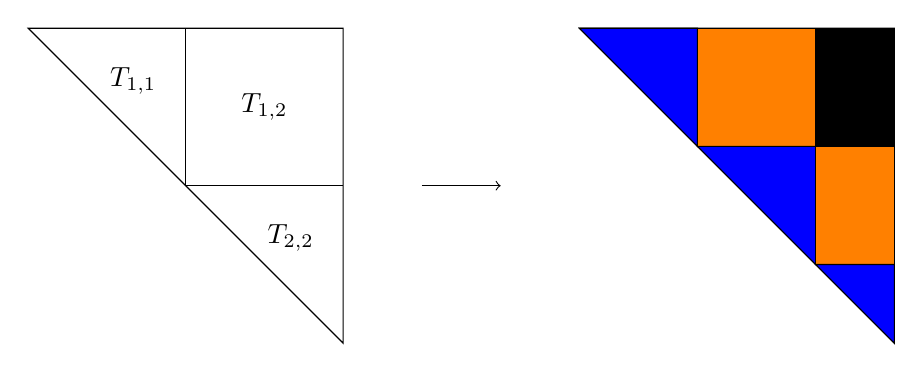
\begin{tikzpicture}
            \draw  (4,4) % Top right
                -- (4,0) % bottom right
                -- (0,4) % top left
                -- cycle;
            \draw  (2,4)
                -- (2,2)
                -- (4,2);
            \node at (1.333,3.333) {$T_{1,1}$};
            \node at (3,3) {$T_{1,2}$};
            \node at (3.333,1.333) {$T_{2,2}$};
            \draw[->] (5,2) -- (6,2);
            \draw (7, 4) -- (11,4) -- (11, 0) -- cycle;
            \draw[fill=blue] (7, 4) -- (8.5, 4) -- (8.5, 2.5) -- cycle;
            \draw[fill=orange]  (8.5,4) -- (10,4) -- (10,2.5) -- (8.5,2.5) -- cycle;
            \draw[fill=blue] (8.5,2.5) -- (10, 2.5) -- (10, 1) -- cycle;
            \draw[fill=orange] (10,2.5) -- (11,2.5) -- (11,1) -- (10,1) -- cycle;
            \draw[fill=blue] (10,1) -- (11,1) -- (11,0) -- cycle;
            \draw[fill=black] (10,4) -- (11,4) -- (11,2.5) -- (10,2.5) -- cycle;
        \end{tikzpicture}
    \end{frame}
    \begin{frame}
        \frametitle{Visual Representation Of Terminating Case}
        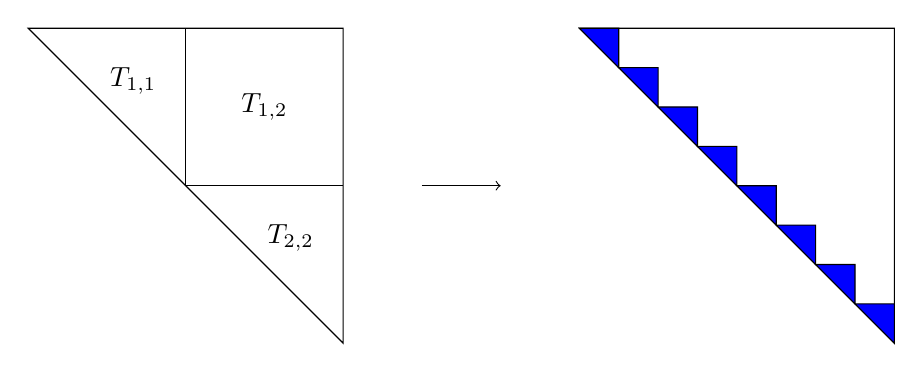
\begin{tikzpicture}
            \draw  (4,4) % Top right
                -- (4,0) % bottom right
                -- (0,4) % top left
                -- cycle;
            \draw  (2,4)
                -- (2,2)
                -- (4,2);
            \node at (1.333,3.333) {$T_{1,1}$};
            \node at (3,3) {$T_{1,2}$};
            \node at (3.333,1.333) {$T_{2,2}$};
            \draw[->] (5,2) -- (6,2);
            \draw (7, 4) -- (11,4) -- (11, 0) -- cycle;
            \draw[fill=blue] (7,4) -- (7.5,4) -- (7.5,3.5) -- cycle;
            \draw[fill=blue] (7.5,3.5) -- (8.0, 3.5) -- (8.0, 3.0) -- cycle;
            \draw[fill=blue] (8.0,3.0) -- (8.5, 3.0) -- (8.5, 2.5) -- cycle;
            \draw[fill=blue] (8.5,2.5) -- (9, 2.5) -- (9, 2) -- cycle;
            \draw[fill=blue] (9,2) -- (9.5, 2) -- (9.5, 1.5) -- cycle;
            \draw[fill=blue] (9.5,1.5) -- (10, 1.5) -- (10, 1) -- cycle;
            \draw[fill=blue] (10,1) -- (10.5, 1) -- (10.5, .5) -- cycle;
            \draw[fill=blue] (10.5, .5) -- (11, .5) -- (11, 0) -- cycle;
        \end{tikzpicture}
    \end{frame}
    \subsection{Matrix Operation LARFT}
    \begin{frame}
        \frametitle{DLARFT\_MAT}
        % Add proper citation to these
        Based on the work done by Joffrain and et. al. \footnote{Accumulating Householder Transformations, Revisited} and Puglisi \footnote{Modification of the Householder method based on the compact wy representation}
        \\\,\\
        \begin{algorithmic}[1]
            \State $T = V^\top V$ (Only upper triangular part)
            \State Scale the diagonal by $\frac{1}{2}$.
            \State $T = T^{-1}$.
        \end{algorithmic}
        \,\\\,\\
        For more details about why this works, see either Theorem 2 from Joffrain et. al. or the algorithm from Puglisi
    \end{frame}
    \subsection{Numerical Experiments}
    \begin{frame}
        \frametitle{Numerical Results}
        We ran the following tests on the Alderaan\footnote{Specifications for the cluster can be found 
        \textcolor{blue}{\href{https://ccm-docs.readthedocs.io/en/latest/alderaan\#hardware}{here}}\\\,} 
        cluster here at UC Denver\\
        % put pictures here of just the times.
        \begin{center}
        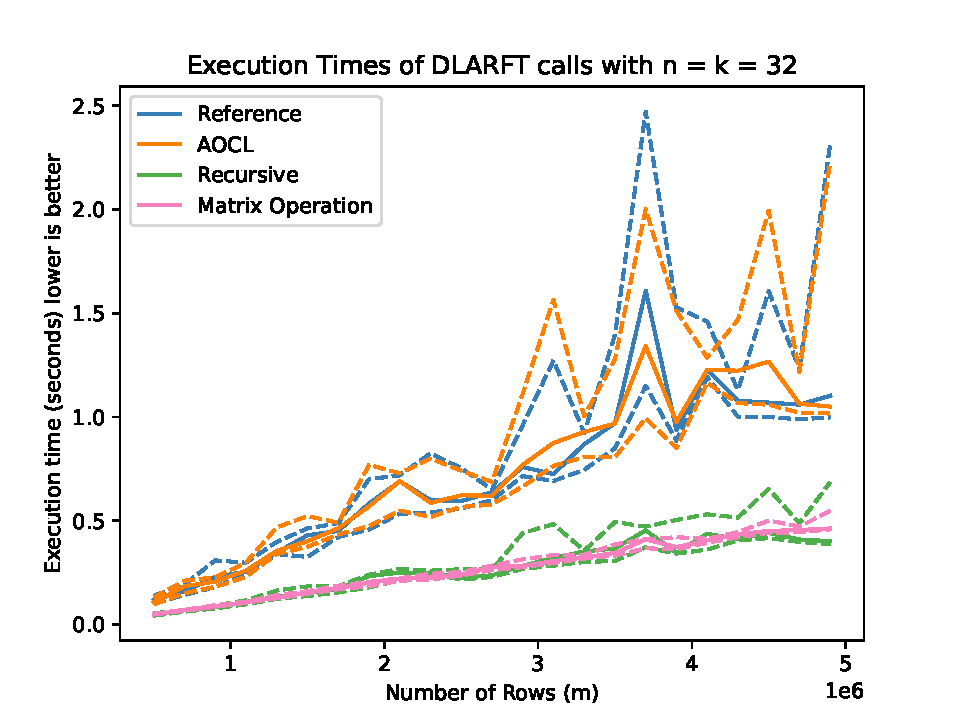
\includegraphics[width=.45\textwidth]{figures/timeDLARFT.pdf}
        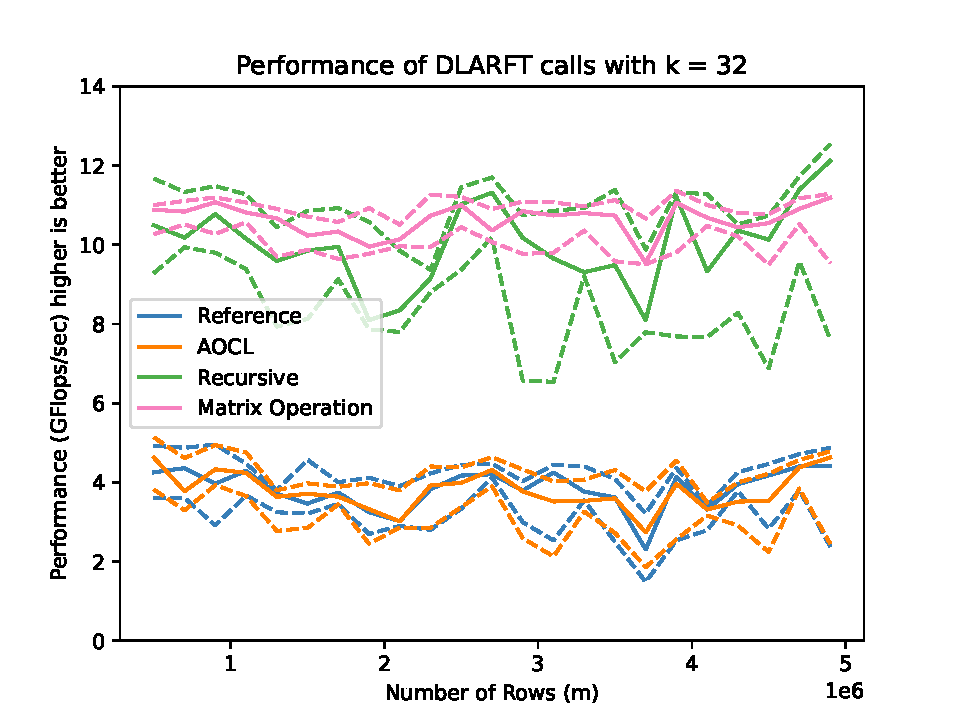
\includegraphics[width=.45\textwidth]{figures/flopDLARFT.pdf}
        \end{center}
    \end{frame}
    \subsection{Computational Cost}
    %\begin{framefont}{\small}
    \begin{frame}
        \frametitle{Floating Point Operation Count}
        For these two different versions, we get the following computation cost for $V\in\R^{m\times n}$ and  $T\in\R^{n\times n}$
        $$
        \begin{aligned}
            \text{DLARFT: }&\,      \frac{6mn^2 - 6mn -4n^3 +6n^2 - 2n}{6}&\approx mn^2\\
            \text{DLARFT\_REC: }&\, \frac{6mn^2 - 6mn -2n^3 +3n^2 -  n}{6}&\approx mn^2\\
            \text{DLARFT\_MAT: }&\, \frac{6mn^2 + 6mn +4n^3 -9n^2 + 5n}{6}&\approx mn^2 
        \end{aligned}
        $$
        Even though in both of our new versions, we have more operations, these are almost all on the order of $n^3$, 
        which we assume is a constant.
        % Roughly 10k more operations, which is nothing for modern machines. We are on fractions of a second with this
        %   number
    \end{frame}
    %\end{framefont}
    \section{DLARFB}
    \begin{frame}
        \frametitle{DLARFB Algorithm}
        Want to compute $C = HC$ where $H$ has the form
        $$
        H = I - VTV^\top
        $$
        And $C$ is any matrix of the proper shape. We break up $V$ and $C$ as follows
        $$
            V = \begin{bmatrix}
                V_1\\
                V_2
            \end{bmatrix} \qquad
            C\footnote{We will also have two specialized routines for when $C_1 = 0$ and one with $C_1=0$ and $C_2=I$} = \begin{bmatrix}
                C_1\\
                C_2
            \end{bmatrix}.
        $$
    \end{frame}
    \begin{frame}
        \frametitle{DLARFB Algorithm}
        By doing so, and doing some algebra, we get the following two updates we need to compute, which are
        \begin{align*}
            C_1 &= C_1 - V_1T\left(V_1^\top C_1 + V_2^\top C_2\right) \\
            C_2 &= C_2 - V_2T\left(V_1^\top C_1 + V_2^\top C_2\right)
        \end{align*}
    \end{frame}
    \subsection{Existing behavior}
    \begin{frame}
        \frametitle{Current Algorithm}
        %Assuming that $C$ is non-zero, we need an extra bit of memory of size $nb\times nb$.
        Reference LAPACK does the following with a workspace of size $nb\times nb$ denoted $W$\\\,\\
        \begin{algorithmic}[1]
            \State $W = C_1^\top$
            \State $W = WV_1$
            \State $W = W + C_2^\top V_2$
            \State $W = WT^\top$
            \State $C_2 = C_2 - V_2W^\top$
            \State $W = WV_1^\top$
            \State $C_1 = C_1 - W^\top$
        \end{algorithmic}\,\\
        However, we get an extra bit of information in this function that $C_1$ starts as the $0$ matrix, which is the correct
        size, so we can use that as a workspace instead!
    \end{frame}
    \subsection{New Behavior}
    \begin{frame}
        \frametitle{New algorithm}
        Taking advantage of the fact that for DORGQR, $C_1 = 0$, we have the following sequence of operations
        \begin{algorithmic}[1]
            \State $C_1 = V_2^\top C_2$
            \State $C_1 = TC_1$
            \State $C_2 = C_2 - V_2C_1$
            \State $C_1 =     - V_1C_1$
        \end{algorithmic}
    \end{frame}
    \subsection{Flop Comparison}
    \begin{frame}
        \frametitle{Floating Point Operation Counts}
        For these two different versions, we get the following computation cost for $V\in\R^{m\times k}$, $T\in\R^{k\times k}$, and $C\in\R^{m\times n}$.\footnote{Note: In our actual loops, we grow $m$ and $n$, and $k$ is the blocking parameter usually just set to $32$.}
        \begin{align*}
            \text{DLARFB: }&\, 4mnk - nk^2 + nk\\
            \text{NEW\_DLARFB: }&\, 4mnk - 2nk^2
        \end{align*}
        In addition to our memory savings, we also have a slight computation improvement. We don't see
        much of this benefit in computational cost in practice though. Note: we are also linear in $m$ and
        $n$, so we scale well when we treat $k$ as a constant blocking parameter.
    \end{frame}
    \begin{frame}
        \frametitle{Numerical Experiments}
        \begin{center}
        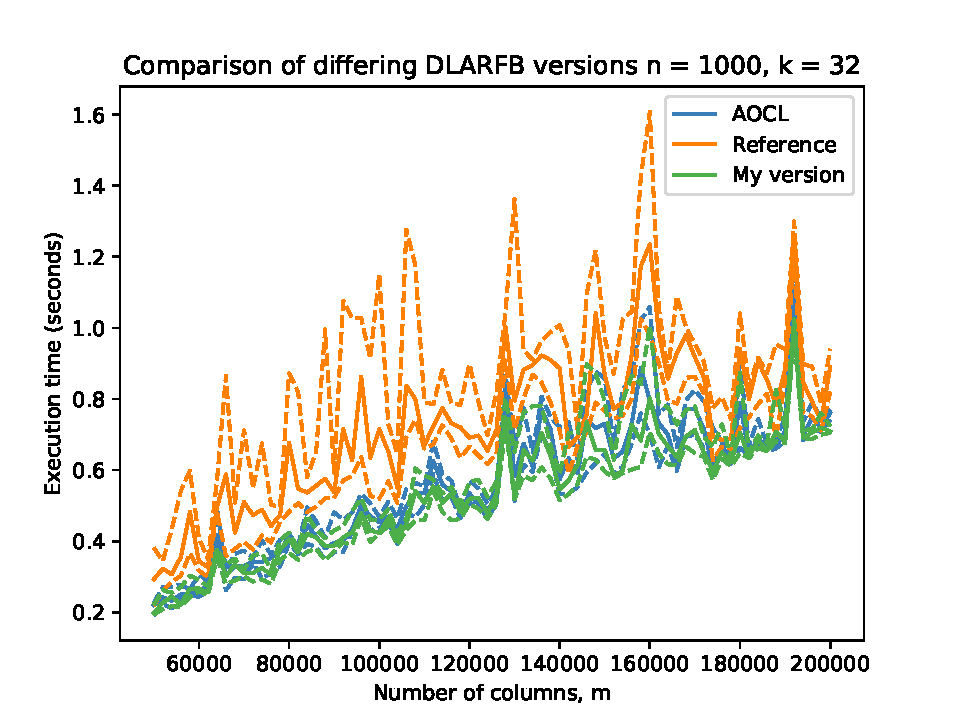
\includegraphics[width=.45\textwidth]{figures/timeDLARFB.pdf}
        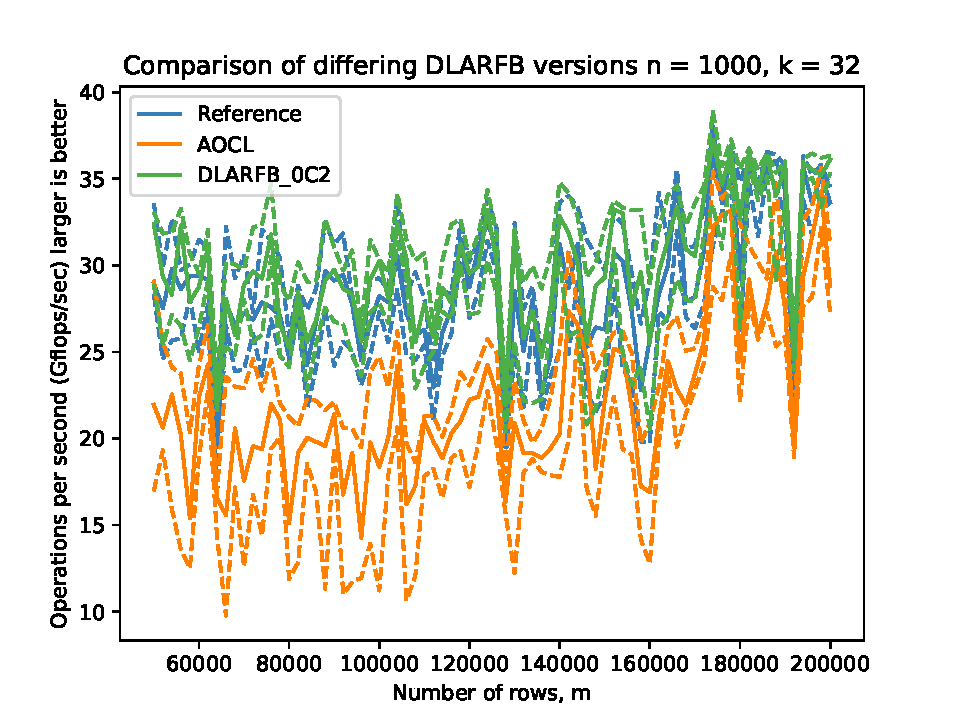
\includegraphics[width=.45\textwidth]{figures/flopDLARFB.pdf}
        \end{center}
    \end{frame}
    \section{Main Driver Algorithm}
    \subsection{Saving Flops on first iteration}
    \begin{frame}
        \frametitle{Initial Savings}
        If we refer back to the algorithm of DLARFB, we can take advantage in our first step having $C_1 = 0$ and $C_2=I$. So 
        the first step can be rewritten as
        \begin{algorithmic}[1]
            \State $C_1 = TV_2^\top$
            \State $C_2 = C_2 - V_2C_1$
            \State $C_1 =     - V_1C_1$
        \end{algorithmic}
        This saves a DGEMM call, which is one the most expensive operation inside DLARFB
    \end{frame}
    \section{DORG2R}
    \subsection{What it is supposed to do}
    \begin{frame}
        \frametitle{Unblocked version}
        DORG2R is the unblocked version that is based on matrix-vector products instead of matrix-matrix 
        operations. In general, this will be slower for most use cases, but is used in our blocked loop. So, we discuss the general behavior now.
    \end{frame}
    \subsection{Existing Behavior}
    \begin{frame}
        % Summary: This is just DORGQR with a blocksize of 1
        \frametitle{DORG2R algorithm inside DORGQR}
        Reminder: our main algorithm is as follows:
        \begin{algorithmic}[1]
            \For{Each column of $V$ denoted $v_i$}
            \State Apply $I-\tau_iv_iv_i^\top$ to the trailing columns of $Q$
            \EndFor
        \end{algorithmic}
        This ends up being much slower as we are doing matrix vector operations, which are not as
        efficient as matrix-matrix operations
    \end{frame}
    \subsection{``Blocked'' equivalent}
    \begin{frame}
        \frametitle{What about a middle ground?}
        Since we already have our $T$ computed, why not try to use it to make the last application of our reflectors
        more efficient! Since we are assuming $T$ is a ``small'' matrix, we can manually compute 
        $$
            I - VTV^\top
        $$
        without having to loop!
    \end{frame}
    \section{DORGKR}
    \subsection{Algorithm Overview}
    \begin{frame}
        \frametitle{DORGKR Algorithm}
        $$
            Q = I - VTV^\top
        $$ where
        $$
        V = \begin{bmatrix} V_1 \\ V_2 \end{bmatrix}
        Q = \begin{bmatrix} Q_1 \\ Q_2 \end{bmatrix}
        $$
        \begin{algorithmic}[1]
            \State $T = TV_1^\top$
            \State $Q_2 = -V_2T$
            \State $Q_1 = -V_1T$
            \State $Q = I - Q$
        \end{algorithmic}
    \end{frame}
    \subsection{Numerical Experiments}
    \begin{frame}
        \frametitle{Comparison of DORGKR to DORG2R}
        %more improvement from the fact that we are blocking and using matrix-matrix operations,
        %which are much faster in practice.
        \begin{center}
        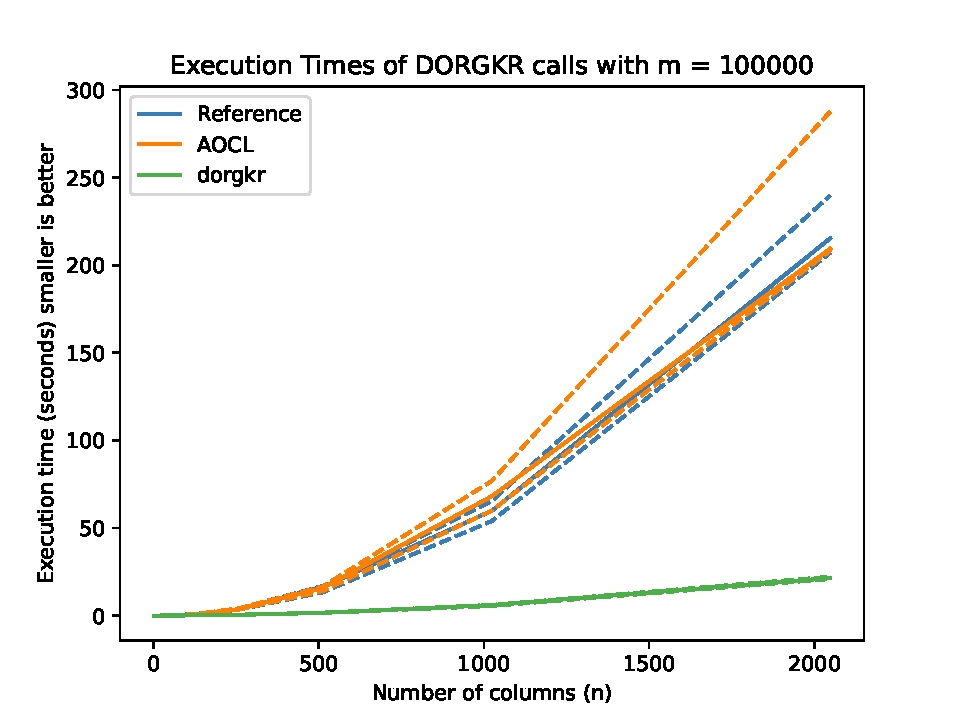
\includegraphics[width=.45\textwidth]{figures/timeDORGKR.pdf}
        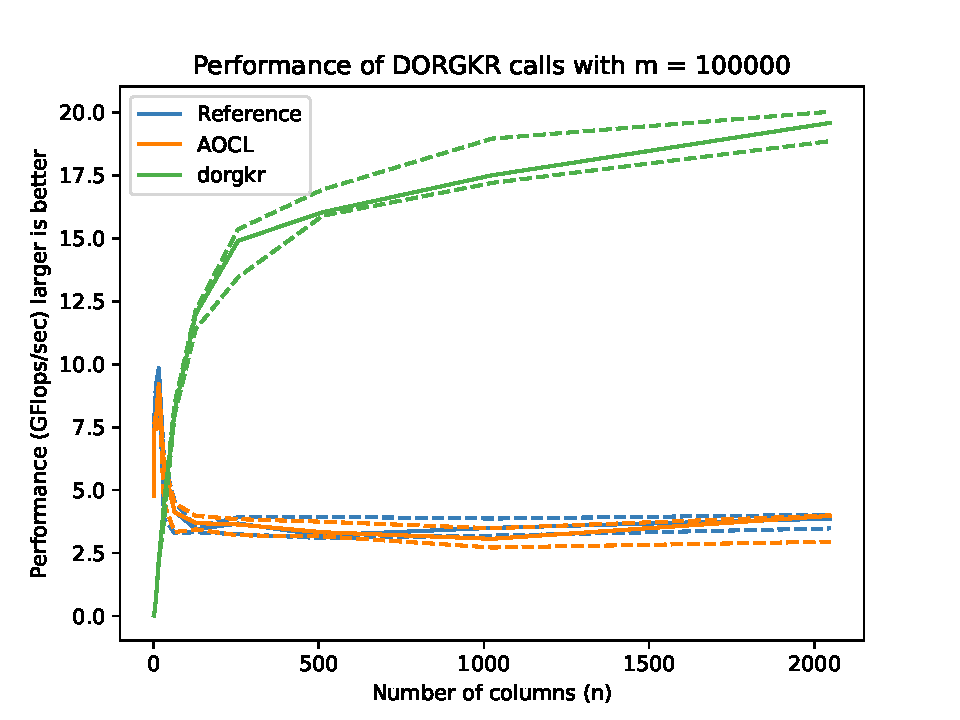
\includegraphics[width=.45\textwidth]{figures/flopDORGKR.pdf}
        \end{center}
    \end{frame}
    \subsection{Computational Cost}
    \begin{frame}
        \frametitle{Floating Point Operation Cost}
        Assuming we have $V\in\R^{m\times n}$ and $T\in\R^{n\times n}$ our costs are 
        $$
        \begin{aligned}
            % Note: This is only true for the k = n case for DORG2R
            \text{DORG2R: }&\, \dfrac{12mn^2 - 6mn -4n^3 +9n^2 - 11n}{6} &\approx 2mn^2\\
            \text{DORGKR: }&\, \dfrac{2mn^2 + n^2 - n}{2} &\approx mn^2
        \end{aligned}
        $$
        We see an improvement for a factor of $2$, which is non-negligbile, but we should note that the sizes
        used within our routine are relatively small, so we won't see this improvement much when we put it all together

        
    \end{frame}
    \section{Putting it all together}
    \begin{frame}
        \frametitle{My DORGQR vs Existing DORGQR} 
        When putting all the above pieces together, we see the following performance

        We omit the FLOP counts for these routines as they introduce another variable and another question that we don't
        have time to discuss in detail. % vary m=n, vary k vs vary m, vary n=k
        \begin{center}
        %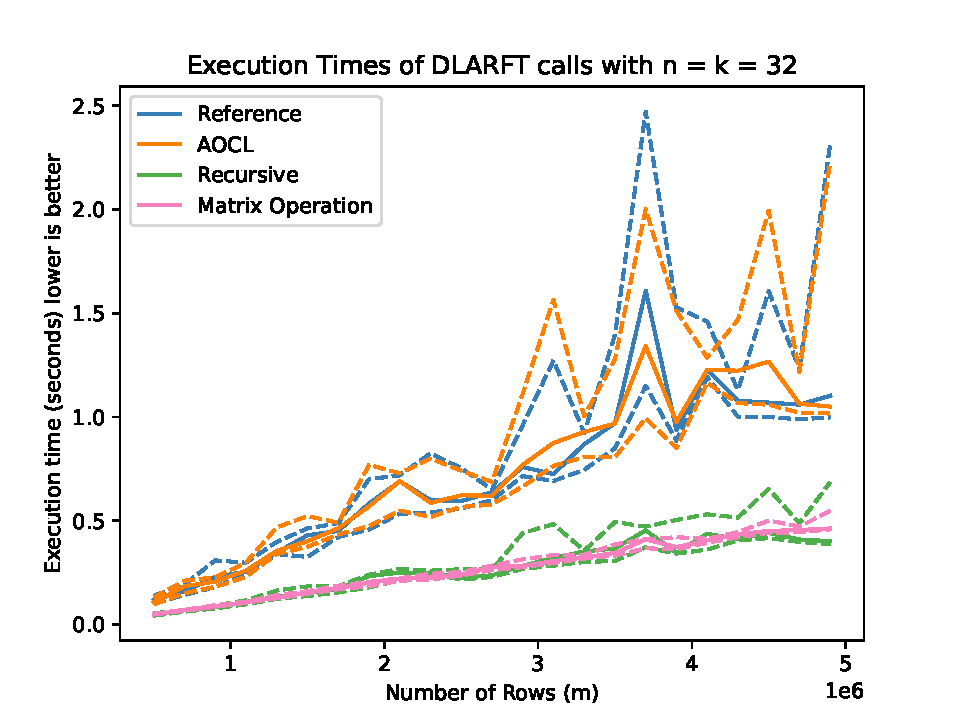
\includegraphics[width=.45\textwidth]{figures/timeDLARFT.pdf}
        %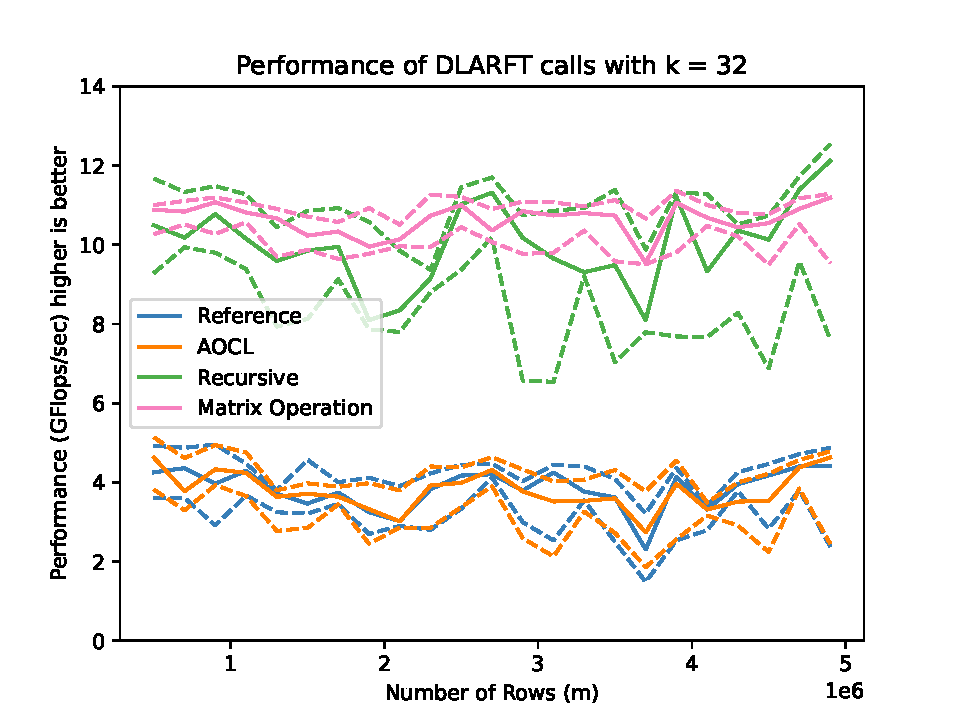
\includegraphics[width=.45\textwidth]{figures/flopDLARFT.pdf}
        \end{center}
        \textbf{\large Need to regenerate these. Issue in timing files. Will use much smaller cases to get something for this slide}
    \end{frame}
    \section{References}
    \begin{frame}
        \frametitle{References}
    \end{frame}
    \begin{frame}
        \frametitle{Thanks for listening!}
        Are there any questions?
    \end{frame}

\end{document}
